\documentclass[10pt]{article}
\usepackage[margin=1in]{geometry}
\usepackage{amsmath,amssymb,amsthm}
\usepackage{pstricks}
\usepackage{wrapfig}
\usepackage{graphicx}
\usepackage{fancyhdr}
\pagestyle{fancyplain}
\usepackage{lastpage}
\usepackage{hyperref}

\newcommand{\mytitle}{Applications}
\newcommand{\myclass}{Math 341}

\rhead{pg. \thepage  \ of \pageref{LastPage}}    
\chead{\myclass}
\lhead{\mytitle}
\lfoot{\noindent(Draft \today)}
\cfoot{}



%The purpose of this code is to allow me to put lines in matrices so that I can create augmented matrices.
\makeatletter
\renewcommand*\env@matrix[1][*\c@MaxMatrixCols c]{%
  \hskip -\arraycolsep
  \let\@ifnextchar\new@ifnextchar
  \array{#1}}
\makeatother

\newcommand{\ds}{\displaystyle}

\begin{document}


\noindent{\huge{\bf \mytitle}}

\noindent
This learning module covers the following ideas.  When you make your lesson plan, it should explain and contain examples of the following:
\begin{enumerate}

\item Use Gaussian elimination to find least degree interpolating polynomials, compute partial fraction decompositions, and solve for electrical currents in electrical systems involving batteries and resistors.
\item Explain how to generalize the derivative to a matrix. Use this generalization to approximate changes in a function and locate optimal values of the function using the second derivative test.
\item Describe a Markov Process, and connect it to powers of a square matrix. Explain how eigenvectors are related to limits of Markov Processes.
\item Find bases of vectors for the row and column spaces of a matrix. Explain how to decompose a matrix into the product of matrices involving these bases, and how to each row and column of your matrix can be expressed as a linear combination of these bases.
\item Use the transpose and inverse of a matrix to solve the least squares regression problem of fitting a line to a set of data. Describe and illustrate Cramer's rule, and use it to obtain a complete solution to the least squares problem.
\end{enumerate}


Following you will find preparation assignments and suggested homework, and then my best attempt at condensing the information we are learning into a concise set of notes.  For this unit, these are intended to be a complete set of notes.  The homework for this unit is found in the accompany applications problems. As you read my notes, please do the examples yourself and then find examples like them in the homework. With these notes I am trying follow the model found in ``Preach My Gospel,'' where the gospel is taught in a complete concise manner, with suggestions provided for additional study and practice.

\section{Preparation and Suggested Homework}
As a group of 4, each of you should select one of the following problems. To be prepared for class, you should complete the problem you selected and come to class prepared to show your group how that problem is solved.  Occasionally you will be asked to teach this problem to your group, but usually we will attempt similar problems in class. By coming prepared, you will serve as a mini expert group in your group.  If you have spent 20-30 minutes on the problem, looked for and tried similar problems (including the online solutions), and are still stuck, then count yourself as prepared. I strongly suggest that you attempt all the others problems (5 minutes with each is sufficient) before coming to class. If you do not understand a problem, that is OK; it means you are learning and have questions that we can answer in class. This preparation activity should take no more than 30 minutes of your time.  Please use the rest of your time to solve other homework problems related to what we are learning, and complete corrections as needed.

\begin{center}
\begin{tabular}{ll}
&Preparation Problems\\
\hline\hline
Day 1& 2 , 7, 13, 14\\ \hline
Day 2& 23, 29, 37, 41\\ \hline
Day 3& 49, 51, 54, 65\\ \hline
\end{tabular}
\end{center}


The homework problems for this unit come from the accompanying applications problems list.  I strongly suggest that you do 2-3 of each type of problem. The technology introduction contains step-by-step solutions for many of the problems, so that you can check your work.  I will be spending the next few days creating handwritten solutions for many of the problems.

\textbf{
Minimum Homework Goal: 28 
- Minimum Technology Goal: 8 
}
(You should do at least 28 problems, at least 8 of which you solved using Maple. You will report what you have done via a stewardship report.)      



\section{Solving Systems}
\subsection{Fitting a Polynomial}
Through any two points (with different $x$ values) there is a unique line of the form $y=mx+b$. If you know two points, then you can use them to find the values $m$ and $b$.  Through any 3 points (with different $x$ values) there is a unique parabola of the form ($y=ax^2+bx+c$), and you can use the 3 points to find the values $a,b,c$.  As you increase the number of points, there is still a unique polynomial with degree one less than the number of points, and you can use the points to find the coefficients of your polynomial.  In this section we will illustrate how this is done, and how the solution results in a linear system. 

In order to organize our work, we first standardize the notation.  Rather than writing $y=mx+b$, we write $y=a_0+a_1 x$ (where $a_0=b$ and $a_1=m$).  For a parabola, we write $\ds y=a_0 + a_1 x+ a_2 x^2 = \sum_{k=0}^{2} a_k x^k$. This allows us to write any degree polynomial in the form $\ds y = a_0 + a_1 x+ \cdots + a_n x^n = \sum_{k=0}^n a_k x^k$ (by standardizing what we call the coefficients, we can use summation notation to express any degree polynomial by changing the $n$ on the top of the summation sign).

Now that our notation is organized, let's find a degree 2 polynomial through the three points $(0, 1), (2, 3), (4, 7)$.  The polynomial is $y=a_0 +a_1 x+a_2 x^2$, where our job is to find the three constants $a_0, a_1, a_2$.  Since we have three points, put those points into the equation to obtain the three equations
$$
a_{{0}}=1 \quad \quad 
a_{{0}}+2\,a_{{1}}+4\,a_{{2}}=3 \quad \quad 
a_{{0}}+4\,a_{{1}}+16\,a_{{2}}=7
$$
This is a system with 3 equations and 3 unknowns.  Write the system in matrix form and reduce it.
$$
\begin{bmatrix}[ccc|c] 
1&0&0&1\\
1&2&4&3\\
1&4&16&7
\end {bmatrix}
\xrightarrow{\text{rref}}
\begin{bmatrix}[ccc|c]
1&0&0&1\\
0&1&0&1/2\\
0&0&1&1/4
\end {bmatrix} 
$$
The solution is $a_0 = 1, a_1= 1/2, a_2=1/4$, or $y=1+\frac12 x+ \frac 14 x^2$.  

In the solution above, notice that powers of the $x$ values appear as the coefficients of our coefficient matrix, and we augment that matrix by the $y$ values. This is the general pattern used in finding an interpolating polynomial.  If there are 4 points, then you just add one row and one column to the matrix. The figure below shows the general method for quadratics and cubics.
\begin{center}
\begin{tabular}{|c|c|}
$(x_1,y_1),(x_2,y_2),(x_3,y_3)$ & $(x_1,y_1),(x_2,y_2),(x_3,y_3),(x_4,y_4)$\\
 $
\begin{bmatrix}[ccc|c] 
x_1^0&x_1^1&x_1^2&y_1\\
x_2^0&x_2^1&x_2^2&y_2\\
x_3^0&x_3^1&x_3^2&y_3
\end {bmatrix}
\xrightarrow{\text{rref}}
\begin{bmatrix}[ccc|c]
1&0&0&a_0\\
0&1&0&a_1\\
0&0&1&a_2
\end {bmatrix} 
$
&
$
\begin{bmatrix}[cccc|c] 
x_1^0&x_1^1&x_1^2&x_1^3&y_1\\
x_2^0&x_2^1&x_2^2&x_2^3&y_2\\
x_3^0&x_3^1&x_3^2&x_3^3&y_3\\
x_4^0&x_4^1&x_4^2&x_4^3&y_4
\end {bmatrix}
\xrightarrow{\text{rref}}
\begin{bmatrix}[cccc|c]
1&0&0&0&a_0\\
0&1&0&0&a_1\\
0&0&1&0&a_2\\
0&0&0&1&a_3
\end {bmatrix} 
$\\
 $y=a_0+a_1x+a_2x^2$& $y=a_0+a_1x+a_2x^2+a_3x^3$
\end{tabular}
\end{center}


\subsection{Partial Fraction Decomposition}
A partial fraction decomposition is a method of breaking a complex rational function up into the sum of smaller simpler functions to work with. Some places you will see partial fraction decompositions are in techniques of integration (in math 113) and differential equations (math 316 or math 371). To illustrate their value, let's start with an example.

Let's find the integral of the function $\ds f(x)= {\frac {2x+1}{ \left( x-2 \right)  \left( x-3 \right) }}$. The denominator is the product of two linear functions. Is it possible to break up the function into two simpler functions, namely can we write 
$${\frac {2\,x+1}{ \left( x-2 \right)  \left( x-3 \right) }}={\frac {A}{
x-2}}+{\frac {B}{x-3}}$$
for unknown constants $A$ and $B$? If we multiply both sides by the original denominator, we obtain (cancel the common factors)
$$2x+1 = A(x-3)+B(x-2).$$
Now expand the right hand side and collect the terms which have the same powers of $x$, 
$$2x+1 = (A+B)x+(-3A-2B).$$
Both sides of the equation above represent lines. In order for the two lines to be the same line, they must have the same slope and intercept.  This means we can create an equation for each power of $x$ by equating the coefficients on both sides of the equation.  This gives us the two equations
$$2=A+B \quad \quad 1=-3A-2B.$$
This is now a linear system and we can use Gaussian elimination to solve it as follows:
$$
\begin{bmatrix}[cc|c]
1&1&2\\
-3&-3&1
\end{bmatrix}
\xrightarrow{\text{rref}}
\begin{bmatrix}[cc|c]
1&0&-5\\
0&1&7
\end{bmatrix}
$$
Our solution is $A=-5,B=7$ and we can write ${\frac {2\,x+1}{ \left( x-2 \right)  \left( x-3 \right) }}={\frac {-5}{
x-2}}+{\frac {7}{x-3}}$. We can now integrate each term separately to obtain 
$$\int{\frac {2\,x+1}{ \left( x-2 \right)  \left( x-3 \right) }}dx 
= \int {\frac {-5}{x-2}} dx +\int{\frac {7}{x-3}}dx
= {-5}\ln|{x-2}|+7\ln|{x-3}|.
$$

The general process for finding a partial fraction decomposition requires that you start with an appropriate guess for the final form, multiply both sides by the original denominator, collect like powers of $x$ on both sides, and then solve the corresponding linear system. Provided the denominator can be factored, this process can always be used to obtain an integral of a rational function. In math 113 we discuss how to choose an appropriate guess, and in differential equations partial fraction are used to solve differential equations with Laplace transforms. For the problems on the homework, I will provide the guessed form. Your job will be to find the unknowns constants in the form, and then integrate.

As a final example, let's compute $\int {\frac {-{x}^{2}+2\,x+5}{ \left( {x}^{2}+1 \right)  \left( x-3
 \right) }}dx$, using the form  
$${\frac {-{x}^{2}+2\,x+5}{ \left( {x}^{2}+1 \right)  \left( x-3
 \right) }}={\frac {Ax+B}{{x}^{2}+1}}+{\frac {C}{x-3}}$$
In this case the denominator doesn't factor into a product of linear terms, so the quadratic term $x^2+1$ has a linear term $Ax+B$ in the numerator.  Multiplying both sides by the denominator and collecting powers of $x$ gives
$$-{x}^{2}+2\,x+5= \left( A+C \right) {x}^{2}+ \left( B-3\,A \right) x+(C-3\,B).$$
Equating the coefficients of $x$ on each side gives the three equations 
$$5=C-3B, 2=B-3A, -1=A+C$$
Rewriting in matrix form and reducing the matrix gives us
$$
\begin{bmatrix}[ccc|c] 
0&-3&1&5\\
-3&1&0&2\\
1&0&1&-1
\end {bmatrix}
\xrightarrow{\text{rref}}
\begin{bmatrix}[ccc|c]
1&0&0&-6/5\\
0&1&0&-8/5\\
0&0&1&1/5
\end {bmatrix} .
$$
We can now integrate using our solution to obtain 
\begin{align*}
\int {\frac {-{x}^{2}+2\,x+5}{ \left( {x}^{2}+1 \right)  \left( x-3\right) }}dx
&= \int {\frac{1}{5}\left(\frac {-6x-8}{{x}^{2}+1}\right)}+ \frac{1}{5}\left({\frac {1}{x-3}}\right)dx \\
&= -\frac{6}{5}\int \frac{x}{x^2+1}dx -\frac{8}{5}\int \frac{1}{x^2+1}dx +\frac{1}{5}\int{\frac {1}{x-3}}dx\\
&= -\frac{6}{10}\ln|{x^2+1}| -\frac{8}{5}\arctan x +\frac{1}{5}\ln|{x-3}|+C.
\end{align*}


\subsection{Kirchoff's Electrical Laws}

ERROR IN DIAGRAM. REDO.

Gustav Kirchoff discovered two laws that pertain the conservation of charge and energy in the study of electricity.  In order to describe these laws, we first need to discuss voltage, resistance, and current.  Current is the flow of electricity, and often it can be compared to the flow of water.  Whenever a current passes across a conductor, it encounters resistance. Ohm's law states that the product of the resistance $R$ and current $I$ across a conductor equals the voltage $V$, or $RI=V$. If the voltage remains constant, then a large resistance corresponds to a small current. A resistor is an object with high resistance which is placed in an electrical system to slow down the flow (current) of electricity.  Resistors are measured in terms of ohms, and the larger the ohms, the smaller the current.  The following diagrams illustrate two introductory electrical systems.
\begin{center}\begin{tabular}{cc}
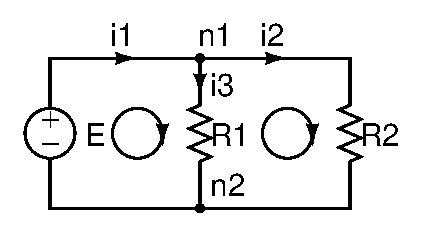
\includegraphics[height=1in]{electric-circuit-1}
&
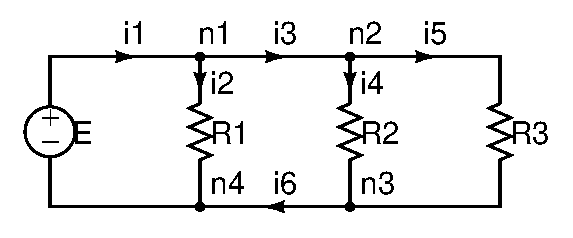
\includegraphics[height=1in]{electric-circuit-2}\\
Two Loop System & Three Loop System
\end{tabular}\end{center}
Wires in this diagram meet at nodes (which are illustrated with a dot, and are labeled with $n$'s).  
Batteries (or voltage sources) are often depicted with the symbol 
\includegraphics[height=10pt]{battery}, and they supply a voltage of $E$ volts. The electrical current on each wire flows away from the positive end of a battery and toward the negative end. At each node the current may change, so the arrows and letters $i$ represent the different currents in the electrical system. Resistors are depicted with the symbol 
\includegraphics[height=10pt]{resistor}, and the letter $R$ represents the ohms. 

Kirchoff discovered two laws. They both help us find current in a system, provided we know the voltage of any batteries, and the resistance of any resistors. 
\begin{enumerate}
	\item Kirchoff's current law states that at every node, the current flowing in equals the current flowing out (at nodes, current in = current out). 
	\item Kirchoff's voltage law states that on any loop in the system, the directed sum of voltages supplied equals the directed sum of voltage drops (in loops, voltage in = voltage out). 
\end{enumerate}

Let's use Kirchoff's laws to generate a system of equations for the two loop system. At the first node ($n_1$), current $i_1$ flows in while $i_2$ and $i_3$ flow out. Kirchoff's current law states that $i_1=i_2+i_3$ or $i_1-i_2-i_3=0$.  At the second node, both $i_2$ and $i_3$ are flowing in while $i_1$ flows out. This means that $i_2+i_3=i_1$ or $-i_1+i_2+i_3=0$. This second equation is the same multiplying both sides of the first by $-1$.  
We now look at Kirchoff's voltage law. Pick a loop and work your way around the loop in a clockwise fashion. Each time you encounter a battery or resistor, include a term for the voltage supplied $E$ on the left side of an equation, and the voltage drop (resistance times current $Ri$) on the right. If you encounter a battery or resistor as you work against the current, then times that term by a negative 1. The left loop has a battery with voltage $E$ and the resistor contributes a drop in voltage of $R_1 i_2$ volts.  An equation for the first loop is $E=R_1i_2$. On the right loop we encounter along the current $i_3$ a resistor with resistance $R_2$ ohms.  While working our way up $i_2$ (against the flow), we encounter a $R_1$ ohm resistor.  There are no batteries. This gives us the equation $0=-R_1 i_2 +R_2i_3$. We can now write a system of equations involving the unknowns $i_1,i_2,i_3$, put it in matrix form and solve
$$\begin{cases}
i_1-i_2-i_3=0\\
-i_1+i_2+i_3=0\\
R_1i_2=E\\
-R_1 i_2 +R_2i_3=0
\end{cases}
\xrightarrow{\text{matrix form}}
\begin{bmatrix}[ccc|c]
1&-1&-1&0\\
-1&1&1&0\\
0&R_1&0&E\\
0&-R_1&R_2&0
\end{bmatrix}
\xrightarrow{\text{rref}}
\begin{bmatrix}[ccc|c]
1&0&0&\frac{E}{R_1}+\frac{E}{R_2}\\
0&1&0&\frac{E}{R_1}\\
0&0&1&\frac{E}{R_2}\\
0&0&0&0
\end{bmatrix}.
$$
The reason we have a row of zeros at the bottom of or system is because the two rows corresponding to the nodes are linearly dependent.  Hence, when we reduce the matrix that dependence relation becomes a row of zeros.

A similar computation can be done for the three loop system. There are 6 unknown currents, 4 nodes, and 3 loops.  This will give us 7 equations with 6 unknowns.  The 4 equations from the nodes will again contribute rows which are linearly dependent. Reduction will give a unique solution. In the homework, you are asked to setup systems of equations for various electrical systems, and then solve them.

\section{Calculus}

\subsection{Differentials and Approximation}

\subsubsection{Differential Notation Review}
The derivative $f^\prime(x)$ is often interpreted as slope at a point. The slope between two points is the rise over the run, the change in $y$ over the change in $x$, or symbolically we write the slope as $\frac{\Delta y}{\Delta x}$ The notation $\frac{dy}{dx}$ conveys the idea that the derivative is really slope at a point.  The notation $dy = f^\prime dx$ reminds us that an actual change $\Delta y$ in a function can be found using the approximation $\Delta y \approx dy = f^\prime dx$.

For example, when constructing a circle of radius 3 inches, the area $A=\pi r^2$ would increase if a manufacturing process instead creates a circle of radius 3.1 inches. By about how much would the area of the circle increase?  The differential $dA = A^\prime dr = 2\pi r dr = 2\pi (2)(.1)= .6\pi\approx 1.88$ gives an approximate increase in the area. The actual increase in the area is $\Delta A = (3.1)^2\pi - (3)^2 \pi\approx 1.92$. Notice that $dA \approx \Delta A$, namely the differential of the area $dA\approx 1.88$ is approximately the same as the actual change in the area $\Delta A\approx 1.92$.

\subsubsection{Functions of the form $\vec f:{\mathbb{R}}^n\to {\mathbb{R}}^m$}
Differential notation is used to study functions with any number of inputs or outputs.  The word function requires that when we write $y=f(x)$, there must be one output $y$ for every input $x$.  In first semester calculus, you study what happens if your inputs and outputs are both numbers. The fact that the input and output are both single numbers is expressed by the notation $f:{\mathbb{R}}\to{\mathbb{R}}$, where ${\mathbb{R}}$ means all real numbers. In this class and beyond, we study what happens if the inputs and outputs are vectors, not just numbers. The notation ${\mathbb{R}}^2$ represents the vectors in the plane, while ${\mathbb{R}}^3$ represents the vectors in space and ${\mathbb{R}}^n$ represents vectors $(x_1,x_2,x_3,\ldots,x_n)$ with $n$ components. 

The function $f(x,y) = 9-x^2-y^2$ has a vector $(x,y)$ of two inputs, and returns a number as its output. We can write $f:{\mathbb{R}}^2\to {\mathbb{R}}^1$ to explicitly remind us about the size of our inputs and outputs. The functions $x=\cos t, y=\sin t$ can be combined into one function $\vec r(t) = (\cos t,\sin t)$ where we input one variable $t$ and get out a vector $(x,y) = (\cos t,\sin t)$ with two components.  The notation $\vec r(t):{\mathbb{R}}^1\to {\mathbb{R}}^2$ reminds us of the size of the inputs and outputs. 

In multivariable calculus, we study functions of the form $\vec f:{\mathbb{R}}^n\to {\mathbb{R}}^m$ for $n,m\leq 3$, and learn many uses of these functions.  In linear algebra, we will study ``linear'' functions of the form $\vec f:{\mathbb{R}}^n\to {\mathbb{R}}^m$ for any finite $n,m$.

\subsubsection{Partial Derivatives}

Recall the derivative of a function with one input is defined to be $\ds \frac{d f}{dx} = \lim_{h\to 0}\frac{f(x+h)-f(x)}{h}$. The derivative gives the best possible linear approximation to changes in a function. This idea is represented by the equation $\Delta  y \approx f^\prime(x)\Delta x$, or in differential form we write $d y=f^\prime(x) dx$.  An equation of a tangent line is found by noticing that a change in $y$ is approximately $y-f(c)$ when the change in $x$ is $x-c$, so the differential form $dy=f^\prime dx$ becomes $(y-f(c))=f^\prime(c)(x-c)$.

If a function has more than one input variable, then division by the vector $\vec h$ is not well-defined, so we run into a problem with generalizing derivatives.  Instead, we compute partial derivatives which approximate change in the function if we hold all other variables constant and just differentiate with respect to one variable.  For the function $f(x,y)$, we define the partial derivative of $f$ with respect to $x$ as $\ds f_x(x,y)=f_x = \frac{\partial f}{\partial x}= \lim_{h\to 0}\frac{f(x+h,y)-f(x,y)}{h}$, and the partial derivative of $f$ with respect to $y$ as $\ds f_y(x,y)=f_y =\frac{\partial f}{\partial y}= \lim_{k\to 0}\frac{f(x,y+k)-f(x,y)}{k}$. Notice that $f_x$ computes a limit as $y$ is held constant and we vary $x$. 

For $f(x,y)=3x^2+4xy+\cos(xy)+y^3$, we obtain $f_x=6x+4y-y\sin(xy)+0$ and $f_y=0+4x-x\sin(xy)+3y^2$. Partial derivatives are found by holding all other variables constant, and then differentiating with respect to the variable in question.

\subsubsection{The Derivative}
The derivative of a function $\vec f:\mathbb{R}^n\to\mathbb{R}^m$ is an $m\times n$ matrix written $D\vec f(\vec x)$, where the columns of the matrix are the partial derivatives of the function with respect to an input variable (the first column is the partial derivative with respect to the first variable, and so on). Some people call this derivative the ``total'' derivative instead of the derivative, to emphasize that the ``total'' derivative combines the ``partial'' derivatives into a matrix. This definition of the derivative gives the best possible linear approximation to changes in a function.



Some examples of functions and their derivative follow. Remember that each input variable corresponds to a column of the matrix.   
\begin{center}
\begin{tabular}{|l|l|}
\hline
Function&Derivative\\ \hline
{$f(x)=x^2$}& {$Df(x) = \begin{bmatrix}2x\end{bmatrix} $}\\ \hline
{$\vec r(t) = \left<3\cos(t),2\sin(t)\right>$}&  {$D\vec r(t) = \begin{bmatrix}-3\sin t\\ 2\cos t\end{bmatrix} $}\\ \hline
{$\vec r(t) = \left<\cos(t),\sin(t),t\right>$}&  {$D\vec r(t) = \begin{bmatrix}-\sin t \\ \cos t \\ 1\end{bmatrix} $}\\ \hline
{$f(x,y)=9-x^2-y^2$}&  {$Df(x,y) =\nabla f(x,y) = \begin{bmatrix}-2x & -2y\end{bmatrix} $}\\ \hline
{$f(x,y,z)=x^2+y+xz^2$}&  {$Df(x,y,z) = \nabla f(x,y,z) = \begin{bmatrix}2x+z^2 & 1 &2xz\end{bmatrix} $}\\ \hline
{$\vec F(x,y)=\left<-y,x\right>$}&  {$D\vec F(x,y) = \begin{bmatrix}0&-1\\ 1&0\end{bmatrix} $}\\ \hline
{$\vec F(r,\theta,z)=\left<r\cos\theta,r\sin\theta,z\right>$}&  {$D\vec F(r,\theta,z) = 
\begin{bmatrix}
\cos \theta &-r\sin\theta&0\\ 
\sin\theta&r\cos\theta&0\\ 
0&0&1
\end{bmatrix} $}\\ \hline
{$\vec r (u,v)=\left<u,v,9-u^2-v^2\right>$}&  {$D\vec r(u,v) = \begin{bmatrix}1&0\\ 0&1\\ -2u&-2v\end{bmatrix} $}\\ \hline
\end{tabular}
\end{center}

\subsubsection{Approximation}
To emphasize that the derivative is the best possible linear approximation to changes in a function, replace $f^\prime$ in the single variable equation $dy=f^\prime dx$ with the derivative $D\vec f(\vec x)$ to obtain $d\vec y =D\vec f(\vec x)d\vec x$ ($d[\text{outputs}]=D\vec f d[\text{inputs}]$).  For a function $z=f(x,y)$ we obtain $dz=Df(x,y)\begin{bmatrix}dx\\dy\end{bmatrix} = \begin{bmatrix}f_x&f_y\end{bmatrix}\begin{bmatrix}dx\\dy\end{bmatrix} = f_xdx+f_ydy$ using matrix multiplication. 

Suppose a manufacturing company wants to create a cylinder with a 1 inch radius, and 5 inches tall (something like a soda can). If the machine makes cylinders which have a 1.1 inch radius and are 4.8 inches tall, how much will that affect the volume of soda that can be put inside the can? Using differential notation, we write $V=\pi r^2 h,r=1,h=5,dr=.1,dh=-.2$. The derivative of volume is the matrix $DV(r,h) = \begin{bmatrix}V_r& V_h\end{bmatrix} =   \begin{bmatrix}2\pi r h& \pi r^2\end{bmatrix}$.  The approximate change in volume is 
$$dV 
= DV \begin{bmatrix}dr\\dh\end{bmatrix} 
= \begin{bmatrix}2\pi r h& \pi r^2\end{bmatrix}\begin{bmatrix}dr\\dh\end{bmatrix}
= \begin{bmatrix}10\pi& \pi\end{bmatrix}\begin{bmatrix}.1\\-.2\end{bmatrix}
= \pi-.2\pi = .8\pi \approx2.5133.
$$
The actual change in volume is $\pi (1.1)^2(4.8) - \pi(1)^2(5) \approx 2.5384$. The actual change is pretty close to the estimated change.  

Let's now look at an example where the number of outputs is more than 1. Consider the equations $x=t+1$ and $y=t^2$, or in vector form $\vec r(t) = \left<t+1,t^2\right>$. This vector equation models the path of an object as it moves through the plane.  At $t=3$, the object is at $\vec r(3) = \left<3+1,3^2\right> =   \left<4,9\right>.$ About where will the object be at $t=3.1$? Differentials say $d\vec r = D\vec r dt$, or 
$$d\vec r
=\begin{bmatrix}dx \\ dy \end{bmatrix} 
=  \begin{bmatrix}1 \\ 2t \end{bmatrix}dt 
=  \begin{bmatrix}1 \\ 6 \end{bmatrix}(.1) 
=  \begin{bmatrix}.1 \\ .6 \end{bmatrix} .
$$
This means the $x$ value has increased .1 to 4.1, and the $y$ values increase .6 to 9.6.









\subsection{The Second Derivative Test}
Let's start with a review from first semester calculus. If a function $y=f(x)$ has a relative extremum at $x=c$, then $f^\prime(c)=0$ or the derivative is undefined. The places where the derivative is either zero or undefined are called critical values of the function. The first derivative test allows you to check the value of the derivative on both sides of the critical value and then interpret whether that point is a maximum or minimum using increasing/decreasing arguments.  The second derivative test requires you to compute the second derivative at $x=c$. If $f^{\prime\prime}(c)>0$ (the function is concave upwards), then the function has a minimum at $x=c$. If $f^{\prime\prime}(c)<0$ (the function is concave downwards), then the function has a maximum at $x=c$. If $f^{\prime\prime}(c)=0$, then the second derivative test fails. 

The function $f(x) = x^3-3x$ has derivatives $f^\prime = 3x^2-3$ and $f^{\prime\prime}=6x$.  The first derivative is zero when $3(x^2-1)=3(x-1)(x+1)=0$, or $x=\pm 1$.  The second derivative at $x=1$ is $6$ (concave upwards), so there is a minimum at $x=1$.  The second derivative at $x=-1$ is $-6$ (concave downwards), so there is a maximum at that point. 

We're now ready to extend this idea to all functions of the form $f:{\mathbb{R}}^n\to{\mathbb{R}}$ (the output is 1 dimensional, so that it makes sense to talk about a largest or smallest number). We will only consider the case $n=2$, as it simplifies the computations and provides all that is needed to extend to all dimensions. The first derivative test breaks down in every dimension past the first, because there are more than 2 ways to approach a point of the domain (you can't just look at the left side or right side). However, at a local extremum, the derivative is still zero, which often results in solving a system of equations. In higher dimensions, there are three classifications of critical points: maximum, minimum, or saddle point (a point where the tangent plane is horizontal, but in some directions you increase and in other directions you decrease). 

The second derivative test does not break down. Consider the function $z=f(x,y)$. Its derivative $Df(x,y) = \begin{bmatrix}f_x&f_y\end{bmatrix}$ is a function with two inputs and two outputs. The second derivative {$D^2f (x,y)= \begin{bmatrix}f_{xx}&f_{xy}\\f_{yx}&f_{yy}\end{bmatrix} $} is a {$2\times 2$} square matrix called the Hessian of $f$. This matrix will always be symmetric, in that the transpose of the matrix equals itself. The eigenvalues of $D^2f$ give the ``directional'' second derivative in the direction of a corresponding eigenvector. The largest eigenvalue is the largest possible value of the second derivative in any direction. The smallest eigenvalue is the smallest possible value of the second derivative in any direction. The \textbf{second derivative test} is the following. Start by finding all the critical points (places where the derivative is zero). Then find the eigenvalues of the second derivative. 
\begin{enumerate}
	\item If the eigenvalues are all positive at a critical point, then in every direction the function is concave upwards. The function has a minimum at that critical point.  
	\item If the eigenvalues are all negative at a critical point, then in every direction the function is concave downwards. The function has a maximum there.  
	\item If there is a positive eigenvalue and a negative eigenvalue, the function has a saddle point there.  
	\item If either the largest or smallest eigenvalue is zero, then the second derivative test fails. 
\end{enumerate}
Eigenvalues are the key numbers needed to generalize optimization to all dimensions. A proof of this fact is beyond the scope of this class.

For the function {$f(x,y)=x^2+xy+y^2$}, the gradient is $Df = \begin{bmatrix}2x+y&x+2y \end{bmatrix}$, which is zero only at $x=0,y=0$ (solve the system of equations $2x+y=0,x+2y=0$). The Hessian is $D^2f = \begin{bmatrix}2&1 \\1&2\end{bmatrix}$. The eigenvalues are found by solving $0=\det \begin{bmatrix}2-\lambda &1 \\1&2-\lambda \end{bmatrix} = (2-\lambda)^2-1 = 4-4\lambda+\lambda^2 -1 = (\lambda-3)(\lambda-1)$, so $\lambda = 3,1$ are the eigenvalues.  Since both eigenvalues are positive, the function is concave upwards in all directions, so there is a minimum at $(0,0)$.  

For the function {$f(x,y)=x^3-3x+y^2-4y$}, the gradient is $Df = \begin{bmatrix}3x^2-3&2y-4 \end{bmatrix}$, which is zero at $x=1,y=2$ or $x=-1,y=2$. Hence there are two critical points, so we have to find two sets of eigenvalues. The Hessian is $D^2f = \begin{bmatrix}6x&0 \\0&2\end{bmatrix}$. When $x=-1,y=2$, the eigenvalues of $\begin{bmatrix}-6&0 \\0&2\end{bmatrix}$ are $\lambda=-6,2$. Since one is positive and one is negative, there is a saddle point at $(-1,2)$. When $x=1,y=2$, the eigenvalues of $\begin{bmatrix}6&0 \\0&2\end{bmatrix}$ are $\lambda=6,2$. Since both are positive, there is a minimum at $(-1,2)$ (as in every direction the function is concave upwards).











\subsection{Markov Process}


Matrices can be used to model a process called a Markov Process. To fit this kind of model, a process must have specific states, and the matrix which models the process is a transition matrix which specifies how each state will change through a given transition. An example of a set of states is ``open'' or ``closed'' in an electrical circuit, or ``working properly'' and ``working improperly'' for operation of machinery at a manufacturing facility. A car rental company which rents vehicles in different locations can use a Markov Process to keep track of where their inventory of cars will be in the future. Stock market analysts use Markov processes and a generalization called stochastic processes to make predictions about future stock values.

We'll illustrate a Markov Process related to classifying land in some region as ``Residential,'' ``Commercial,'' or ``Industrial.'' Suppose in a given region over a 5 year time span that 80\% of residential land will remain residential, 10\% becomes commercial, and 10\%  becomes industrial.  For commerical land, 70\% remains commercial, 20\% becomes residential, and 10\% becomes industrial.  For industrial land, 70\% remains industrial, 30\% becomes commercial, and 0\% becomes residential.  The ``transition'' matrix for a Markov process (the matrix on the left below) is a matrix where each column relates to one of the ``states,'' and the number in each row is the proportion of the column state that will change to the row state through the transition (where the ordering on row and column states is the same).  
We can calculate the next ``state'' by multiplying a current state by this transition matrix. In the land use model described above, the transition matrix is shown below. If current land use is about 50\% residential, 30\% commercial, and 20\% industrial, then 5 years later the land use is calculated below. 
$$ \begin{array}{rl|c}
&\begin{array}{ccc} R&C&I \end{array} & \\
 \begin{array}{c} \text{to }R\\ \text{to }C\\ \text{to }I \end{array}& 
\begin {bmatrix}  .8&.2&0\\.1&.7&.3\\.1&.1&.7 \end {bmatrix}  &

 \begin {bmatrix} .8&.2&0\\.1&.7&.3\\.1&.1&.7 \end {bmatrix}
 \begin {bmatrix} 50\\30\\20 \end {bmatrix}
 =   \begin {bmatrix} 46\\ 32 \\ 22\end {bmatrix} \\
\multicolumn{2}{c}{\text{Transition Matrix}}&\text{5 Year Projection}
\end{array}.
$$  If the same transitions in land use continue, we multiply the previous projection (state) by the transition matrix to obtain a 10, 15, or 20 year projection for land use as shown below:  
\begin{center}\begin{tabular}{ccc}
$
\begin {bmatrix} .8&.2&0\\.1&.7&.3\\.1&.1&.7 \end {bmatrix}
\begin {bmatrix} 46\\ 32 \\ 22 \end {bmatrix}
 =   \begin {bmatrix} 43.2\\ 33.6 \\ 23.2\end {bmatrix}
$ 
&
$
\begin {bmatrix} .8&.2&0\\.1&.7&.3\\.1&.1&.7 \end {bmatrix}
\begin {bmatrix} 43.2\\ 33.6 \\ 23.2 \end {bmatrix}
 =   \begin {bmatrix} 41.28\\ 34.8\\ 23.92\end {bmatrix}
$ 
&
$
\begin {bmatrix} .8&.2&0\\.1&.7&.3\\.1&.1&.7 \end {bmatrix}
\begin {bmatrix} 41.28\\ 34.8\\ 23.92 \end {bmatrix}
 =   \begin {bmatrix} 39.984\\ 35.664 \\ 24.352\end {bmatrix}
$ 
\\
10 Year Projection 
&15 Year Projection 
&20 Year Projection 
\end{tabular}\end{center}
As we continue to multiply on the left by our transition matrix, each time we add 5 more years to our projection. This projection is valid as long as the same trends continue. Will the projections eventually stabilize, reaching a steady state? 

If $\vec x_0$ is our initial state, then the product $A^n \vec x_0=\vec x_n$ gives us the state after $n$ transitions. What happens in the limit as $n\to \infty$? If the current trends in land use continue, what portion of the land will eventually be in each state. Can we reach a state $\vec x = (R,C,I)$ such that $A \vec x=\vec x$, the next state is the same as the current? If this occurs, then any future transitions will not change the state either. This state $\vec x$ is called a steady-state, since it does not change when multiplied by the transition matrix. Finding a steady state is an eigenvalue problem, as we are looking for a solution to the equation $A\vec x = 1\vec x$ (where the eigenvalue is 1). For any Markov process (where the columns of the matrix sum to 1), the number 1 will always be an eigenvalue. The solution to the problem $\ds\lim_{n\to\infty}A^n \vec x_0$ is a steady state. For our Markov process, an eigenvector (using technology) corresponding to 1 is $\begin{bmatrix}\frac{3}{2}&\frac 32&1\end{bmatrix}^T$. Multiplying by 2  we have $\begin{bmatrix}\frac{3}{2}&\frac 32&1\end{bmatrix}^T$. This means that the ratio of land will be 3 acres residential to 3 acres commercial to 2 acres industrial. To write this in terms of percentages, divide each component by 8 (the sum $3+3+2$) to obtain $3/8:3/8:2/8$ or $37.5\%:37.5\%:25\%$. This is the long term percentages of land use.













\section{Rows and Columns}
\subsection{Row Space and Column Space and Rank}
There are many connections between the rows and columns of a matrix.  This section will illustrate how you can decompose a matrix $A$ into the product of two matrices $C$ and $R$ which tell you how to reconstruct the original matrix $A$ as linear combinations or columns of $C$ or rows of $R$. We'll start with an example, and then describe the general process. Then we will add on some new vocabulary (span, dimension, and basis).


Consider the following matrix and its reduced row echelon form:
\begin{center}\begin{tabular}{cc}
$\begin {bmatrix} 1&2&0\\2&1&3\\0&4&-4 \end {bmatrix}
\xrightarrow{\text{rref}}
\begin {bmatrix} 1&0&2\\0&1&-1\\0&0&0 \end {bmatrix}$  &
$2\begin {bmatrix} 1\\2\\0 \end {bmatrix}
-1\begin {bmatrix} 2\\1\\4 \end {bmatrix}
=\begin {bmatrix} 0\\3\\-4 \end {bmatrix}
$\\
Reduction & Interpretation
\end{tabular}\end{center}
Because there is a column which is not a pivot column, we say that the columns of $A$ are linearly dependent. The third column is not a pivot column, so we can use the number in the reduced row echelon form to write the third column as a linear combination of the first two columns as shown above. The reduced row echelon form tells us precisely how to linearly combine the pivot columns of our matrix to construct the original matrix.  

Let $C$ be the matrix whose columns are the pivot columns of $A$.  Let $R$ be the matrix whose rows are the nonzero rows of the reduced echelon form of $A$.  Then we have $A=CR$.  For the matrix in the previous example, we have  
\begin{center}\begin{tabular}{cccc}
$A=\begin {bmatrix} 1&2&0\\2&1&3\\0&4&-4 \end {bmatrix}$&
$C=\begin {bmatrix} 1&2\\2&1\\0&4 \end {bmatrix}$&
$R=\begin {bmatrix} 1&0&2\\0&1&-1 \end {bmatrix}$&
$\begin {bmatrix} 1&2\\2&1\\0&4 \end {bmatrix}\begin {bmatrix} 1&0&2\\0&1&-1 \end {bmatrix} = \begin {bmatrix} 1&2&0\\2&1&3\\0&4&-4 \end {bmatrix} $.
\end{tabular}\end{center}
Some key observations to make are:
\begin{enumerate}
	\item Every column of $A$ is a linear combination of the pivot columns. 
  \item The columns of $R$ are the coefficients needed to obtain the columns of $A$ as linear combinations of columns of $C$.
       In other words, multiplying by $R$ on the right of $C$ gives us linear combinations of columns of $C$.
  \item Every row of $A$ is a linear combination of the rows of $R$.
	\item The rows of $C$ are the coefficients needed to obtain the rows of $A$ as linear combinations of the rows of $R$.
       In other words, multiplying by $C$ on the left of $R$ gives us linear combinations of rows of $R$.
\end{enumerate}
The following product illustrates the first 2 key observations with regards to columns. Notice how information from the columns of $R$ is used to combine the columns of $C$.
\begin{center}
\begin{tabular}{rlcr}
$\begin {bmatrix} 1&2\\2&1\\0&4 \end {bmatrix}\begin {bmatrix} 1&0&2\\0&1&-1 \end {bmatrix} 
$&$=
\left[ 
\begin{bmatrix}1&2\\2&1\\0&4 \end {bmatrix} \begin {bmatrix} 1\\0 \end {bmatrix}\right.$
&$\begin{bmatrix}1&2\\2&1\\0&4 \end {bmatrix} \begin {bmatrix} 0\\1 \end {bmatrix}$
&$\left. \begin{bmatrix}1&2\\2&1\\0&4 \end {bmatrix} \begin {bmatrix} 2\\-1 \end {bmatrix}\right]$
\\&=
$\left[
1\begin{bmatrix}1\\2\\0 \end {bmatrix}+ 0 \begin{bmatrix}2\\1\\4 \end {bmatrix}\right.$
&$0\begin{bmatrix}1\\2\\0 \end {bmatrix}+ 1 \begin{bmatrix}2\\1\\4 \end {bmatrix}$
&$2\left.\begin{bmatrix}1\\2\\0 \end {bmatrix} -1 \begin{bmatrix}2\\1\\4 \end {bmatrix}
\right]$
\end{tabular}
\end{center}
The following product illustrates the last two key observations with regard to rows. Notice how information from the rows of $C$ is used to combine the rows of $R$.
$$
\begin {bmatrix} 1&2\\2&1\\0&4 \end {bmatrix}\begin {bmatrix} 1&0&2\\0&1&-1 \end {bmatrix} 
=
\begin{bmatrix}
\begin{bmatrix}1&2\end {bmatrix} \begin {bmatrix} 1&0&2\\0&1&-1 \end {bmatrix}\\
\begin{bmatrix}2&1 \end {bmatrix} \begin {bmatrix} 1&0&2\\0&1&-1 \end {bmatrix}\\
\begin{bmatrix}0&4 \end {bmatrix} \begin {bmatrix} 1&0&2\\0&1&-1 \end {bmatrix}
\end{bmatrix}
=
\begin{bmatrix}
1 \begin {bmatrix} 1&0&2 \end {bmatrix} +2 \begin {bmatrix} 0&1&-1 \end {bmatrix}\\
2 \begin {bmatrix} 1&0&2 \end {bmatrix} +1 \begin {bmatrix} 0&1&-1 \end {bmatrix}\\
0 \begin {bmatrix} 1&0&2 \end {bmatrix} +4 \begin {bmatrix} 0&1&-1 \end {bmatrix}
\end{bmatrix}.
$$
In summary, matrix multiplication is a way of creating new matrices as linear combinations of other matrices. It can be viewed either by looking at rows, or by looking at columns.

In the above example, the first two columns formed a linearly independent set, and using them we could obtain every other column of $A$.  The set of all linear combinations of columns of $A$ is called the column space of $A$.  Recall that the span of a set of vectors is all possible linear combinations of those vectors.  So the column space of $A$ is the span of the columns of $A$.  Since every non pivot column of $A$ is a linear combination of $A$, we can say that the column space is the span of the pivot columns of $A$.  This introduces an idea called a basis.  A basis for a vector space is a set of linearly independent vectors whose span is the space we are interested in.  So a basis for the column space is the set of pivot columns. The dimension of a vector space is the number of vectors in a basis.  The dimension of our column space is 2.

In a similar fashion, we define the row space to be the span of the row vectors. If we reduce a matrix $A$ to reduced row echelon form, then every row of $A$ is a linear combination of the nonzero rows of $A$. This means that the row space is spanned by the nonzero rows of the reduced row echelon form. Those vectors are linearly independent and hence form a basis for the row space.  The dimension of the row space is hence 2 as well.

In general, the rank of a matrix always equals the dimension of both the column space and row space. So we could define the rank of matrix to be the dimension of the column space, or the dimension of the row space, or the number of pivots, they are all the same. A basis for the column space is the pivot columns of $A$.  A basis for the row space is the nonzero rows of the reduced row echelon form of $A$.  Using these bases, we can reconstruct the matrix $A$ as a product $CR$ where $C$'s columns are a basis for the column space, and $R$'s rows are a basis for the row space.  We will spend much more time with this idea in future units, as span, basis, and dimension are fundamental ideas in Linear Algebra.

The ideas above work with any size matrix (square or not). Here is a decomposition for a 5 by 7 matrix.  The pivots are in columns 1, 2, 3, and  5. The rref form is the right most matrix (after dropping the row of zeros). The rank is 4. 
$$ \begin{bmatrix} 2&1&0&3&-3&3&2\\1&0&3&4&2&4&4\\0&4&0&4&0&0&4\\0&0&0&0&1&-1&1\\0&1&3&4&0&6&1\end{bmatrix} 
 =  \begin{bmatrix} 2&1&0&-3\\1&0&3&2\\0&4&0&0\\0&0&0&1\\0&1&3&0\end{bmatrix} 
 \begin{bmatrix} 1&0&0&1&0&0&2\\0&1&0&1&0&0&1\\0&0&1&1&0&2&0\\0&0&0&0&1&-1&1\end{bmatrix}
$$
Using the above decomposition, I can write the 7th column as 2 times the first plus 1 times the second plus 1 times the 5th.  I can write the 2nd row of the original matrix as the following linear combination of the reduced row echelon form
$$
1 \begin{bmatrix} 1&0&0&1&0&0&2\end{bmatrix} 
+0 \begin{bmatrix} 0&1&0&1&0&0&1\end{bmatrix}
+3 \begin{bmatrix} 0&0&1&1&0&2&0\end{bmatrix}
+2 \begin{bmatrix} 0&0&0&0&1&-1&1\end{bmatrix}.
$$


\subsection{Linear Regression}

Our final application ask the following question: when a system has no solution, how do you find an approximate solution? In particular, if you have 3 or more points, how do you find a line that is "closest" to passing through these points?  This line, called the least squares regression line, can be used to find trends in many branches of science.  Statistics builds upon this idea to provide powerful tools for predicting the future.

Suppose we want to find a line that is closest to passing through the three points $(0,1),(2,3),(4,6)$.  Since the points are not collinear, there is no such line.  Suppose for a moment that there were a line of the form $y=mx+b$ that did pass through the points.  Plugging our 3 points into the equation $mx+b=y$ gives the system of equations 
$$\begin{cases}b=1\\2m+b=3\\4m+b=6\end{cases}
\xrightarrow{\text{augmented matrix}}
\begin{bmatrix}[cc|c]0&1&1\\2&1&3\\4&1&6\end{bmatrix}
\xrightarrow{\text{matrix form}}
\begin{bmatrix}0&1\\2&1\\4&1\end{bmatrix}
\begin{bmatrix}m\\b\end{bmatrix}
=\begin{bmatrix}1\\3\\6\end{bmatrix}.
$$
Notice that the system can be written in matrix form $A\vec x = \vec b$ where $A$ contains a column of $x$ values and $1$'s and $\vec b$ is a column of $y$ values. If you try to reduce this matrix, you will discover the system is inconsistent (has no solution).  There are more equations than variables, so we call the system over determined. 

Is there a way to reduce the number of rows in our system by using linear combinations of the rows we have, so that the resulting system has only 2 rows? If we multiply on the left by a 2 by 3 matrix, we would obtain a system with 2 rows instead of 3, and the rows of the new matrix would be linear combinations of the rows of our original matrix.  The only 2 by 3 matrix in this problem is the transpose of A.  So lets multiply both sides by the transpose of A:
$$A = \begin{bmatrix}0&1\\2&1\\4&1\end{bmatrix}, 
A^T = \begin{bmatrix}0&2&4\\1&1&1\end{bmatrix}, 
A^T A =\begin{bmatrix}0&2&4\\1&1&1\end{bmatrix}\begin{bmatrix}0&1\\2&1\\4&1\end{bmatrix}= \begin{bmatrix}20&6\\6&3\end{bmatrix}, 
A^T\vec b =  \begin{bmatrix}0&2&4\\1&1&1\end{bmatrix}\begin{bmatrix}1\\3\\6\end{bmatrix} = \begin{bmatrix}30\\10\end{bmatrix}.
$$
The equation $A\vec x = \vec b$ becomes the equation $A^T A \vec x = A^T\vec b$, or $\begin{bmatrix}20&6\\6&3\end{bmatrix} \begin{bmatrix}m\\b\end{bmatrix}=\begin{bmatrix}30\\10\end{bmatrix}$. The solution can then be obtained by reducing $\begin{bmatrix}[cc|c]20&6&30\\6&3&10\end{bmatrix}$ to $\begin{bmatrix}[cc|c]1&0&5/4\\0&1&5/6\end{bmatrix}$, which means the solution is $y=\frac{5}{4}x+\frac{5}{6}.$  Later we will prove that $A^T A$ has an inverse, which means we can write $\vec x = (A^T A)^{-1}A^T \vec b = \begin{bmatrix}1/8&-1/4\\-1/4&5/6\end{bmatrix}\begin{bmatrix}30\\10\end{bmatrix} = \begin{bmatrix}5/4\\5/6\end{bmatrix} $ as the solution to our system. 

In general, a least squares regression problem is solved by (1) assuming the form of a solution ($y=mx+b$), (2) putting your values of $x$ and $y$ into the system to get a matrix equation $A\vec x=\vec b$, (3) multiply both sides by $A^T$, and (4) solving the simplified system (using reduction, inverse, or Cramer's rule - the next section).  

\subsection{Cramer's Rule}

Cramer's rule is a theoretical tool which gives the solution to any linear system $A\vec x = \vec b$ with $n$ equations and $n$ unknowns, provided that there is a unique solution.  Let $D=\det(A)$. Let $D_i$ be the determinant of the matrx formed by replacing the $i$th column of $A$ with $\vec b$.  Then Cramer's rule states that $x_1 = \frac{D_1}{D},x_2 = \frac{D_2}{D},\ldots, x_n = \frac{D_n}{D}$. We will prove it in class with pictures which connect determinants to area. This method of solving a system of equations is doable for 2 by 2 and 3 by 3 systems, but quickly becomes computationally inefficient beyond (as computing determinants is ugly on large matrices). For large systems, it is much faster to use Gaussian elimination.  However, Cramer's rule is a very powerful theoretical idea, and can simplify theoretical computations. We'll look at an example with numbers, and then use it in two theoretical instances.

Let's solve $
\begin {bmatrix} 1&2&0\\-2&0&1\\0&3&-2\end {bmatrix} 
\begin {bmatrix} x_1\\x_2\\x_3\end {bmatrix} 
=  \begin{bmatrix} 2\\-2\\1\end {bmatrix}
$ using Cramer's rule.  
We compute $$ 
D=\begin{vmatrix} 1&2&0\\-2&0&1\\0&3&-2\end {vmatrix}  -11,
D_1=\begin{vmatrix} 2&2&0\\-2&0&1 \\1&3&-2\end {vmatrix}   =-12,
D_2=\begin{vmatrix} 1&2&0\\-2&-2&1 \\0&1&-2\end {vmatrix} =-5, 
D_3=\begin{vmatrix} 1&2&2\\-2&0&-2 \\0&3&1\end {vmatrix} =-2 $$
By Cramer's Rule we have, $x_1=12/11, x_2 = 5/11, x_3 = 2/11$.  Using Gaussian Elimination, we obtain the same solution 
$$ \begin {bmatrix}[ccc|c] 1&2&0&2\\-2&0&1&-2\\0&3&-2&1\end {bmatrix}\xrightarrow{\text{rref}}
\begin {bmatrix}[cccc] 1&0&0&12/11
\\0&1&0&5/11\\0&0&1&2/11\end {bmatrix} 
. $$

To find the inverse of a 2 by 2 matrix $A=\begin{bmatrix}a&b\\c&d\end{bmatrix}$, we need to solve $\begin{bmatrix}[cc|c]a&b&1\\c&d&0\end{bmatrix}$ and $\begin{bmatrix}[cc|c]a&b&0\\c&d&1\end{bmatrix}$.  Cramer's rule gives us the formula $$A^{-1}=
\begin{bmatrix}
\begin{vmatrix}1&b\\0&d\end{vmatrix}/|A|&\begin{vmatrix}0&b\\1&d\end{vmatrix}/|A|\\ \\
\begin{vmatrix}a&1\\c&0\end{vmatrix}/|A|&\begin{vmatrix}a&0\\c&1\end{vmatrix}/|A|\end{bmatrix} 
= \frac{1}{|A|}
\begin{bmatrix}d&-b\\-c&a\end{bmatrix}
$$
This provides a quick way to compute determinants of 2 by 2 matrices. Interchange the diagonal entries, change the sign on the others, and divide by the determinant.

To solve the least square regression problem, we need to solve the problem $A^T A \vec x = A^T b$.  We write the matrices on both sides as 
$$A^T A 
=\begin{bmatrix}x_1&x_2&\cdots &x_n\\ 1&1&\cdots&1 \end{bmatrix} \begin{bmatrix}x_1&1\\x_2&1\\\vdots&\vdots \\x_n&1 \end{bmatrix} = \begin{bmatrix}\sum x_i^2 & \sum x_i \\ \sum x_i & n\end{bmatrix} 
\quad\quad
A^T b = \begin{bmatrix}x_1&x_2&\cdots &x_n\\ 1&1&\cdots&1 \end{bmatrix} \begin{bmatrix}y_1\\y_2\\\vdots \\y_n \end{bmatrix}=\begin{bmatrix}\sum x_iy_i\\\sum y_i\end{bmatrix}.
$$
Cramer's rule then says that our solution is 
$$m=\frac{\begin{bmatrix}\sum x_iy_i & \sum x_i \\ \sum y_i & n\end{bmatrix} }{\begin{bmatrix}\sum x_i^2 & \sum x_i \\ \sum x_i & n\end{bmatrix} } = \frac{n\sum x_iy_i -\sum x_i\sum y_i}{ n\sum x_i^2 -\left(\sum x_i\right)^2} \quad\quad
b=\frac{\begin{bmatrix}\sum x_i^2 & \sum x_iy_i \\ \sum x_i & \sum y_i\end{bmatrix} }{\begin{bmatrix}\sum x_i^2 & \sum x_i \\ \sum x_i & n\end{bmatrix} } = \frac{\sum y_i\sum x_i^2 -\sum x_i\sum x_iy_i}{ n\sum x_i^2 -\left(\sum x_i\right)^2}.
$$
At this point a computer program or spread sheet can quickly compute the coefficients without needing Gaussian elimination. Finding this solution without Cramer's rule is more difficult.

\end{document}

















!!!Basic ideas

I need to have Maple code to illustrate the following:
#Finding a best fit polynomial
#Partial fraction decomposition - using parfrac and using a system (this will be harder, as I have to use coefficients and factor)
#Derivatives and matrix multiplication
#Second derivative test
#Markov Process
#Row and column space
#Regression

It appears there are three key types of applications. 
#The first is just solving systems that are created from problems of interest. Best fit polynomials (just plug and solve), partial fraction decompositions (just plug and solve, and then integrate), and electrical network currents (develop the equation, and show how some rows are combinations of others, meaning you don't need them all).
#The second is the derivative (matrix multiplication), second derivative test (eigenvalues and eigenvectors), and Markov Processes (multiplication and eigenvectors)
#The third looks at row-column decomposition (making references to column combinations in the differential, and row combinations in the network), and then a similar matrix type of multiplication to get regression.  

All of these ideas will briefly be introduced as why they are important, and where they come from. The method to solve will be fairly straight forward. This will be a lot to stomach in 3-4 days.  I think it can be done in 3, 



!!!Homework

Finding a best fit polynomial (solving a system - for linear algebra)
#Find a polynomial of least degree which passes through the following points (do 2, 3, 4)


Partial fraction decomposition
#Write 1/(x-2)(x-3) in the form A/(x-2) + B/(x-3). Then find the integral.
#Write 1/(x-1)(x+3) in the form A/(x-1) + B/(x+3). Then find the integral.
#Write 1/(x)^2(x+3) in the form A/(x) + B/(x)^2 + C/(x+3). Then find the integral.
#Write 1/(x-1)^2(x-2) in the form A/(x-1) + B/(x-1)^2 + C/(x-2). Then find the integral.
#Write 1/(x^2+1)(x-1) in the form Ax+B/(x^2+1) + B/(x-1). Then find the integral.
#Write 1/(x^2+4)(x) in the form (Ax+B)/(x^2+4) + B/(x). Then find the integral.


Electrical Networks - 
Using the diagram in the notes (or repeat here), find the currents in the electrical system with the following configurations
#E=10, R1=5, R2=5
#Do a few three system problems (but please use Maple to solve, as it is a 6 system problem)
#Write down the equations that correspond to the 4 nodes in the 3 system problem, and show that the rank is 3 (in other words, you only need to include 3 nodes, as the fourth is a linear combination of the other 3)



Derivatives (multiplication and introduction to Multivariable calculus)
For each function, find its derivative and total differential using matrix multiplication
#f(x,y)=
#f(x,y)=
#r(t) = x,y
In each of the following scenarios, find the derivative of the function as a matrix, and then use differentials and matrix multiplication to estimate a difference.
#The dimensions of a rectangular box are supposed to be 2 by 3 by 5 feet. By about how much will the volume of the box change if 2 increase to 2.1, 3 increase to 3.2, and 5 decreases to 4.7 inches? Find the derivative of the volume, and use matrix multiplication to estimate the change in volume.
#The radius of a cylindrical metal disc is supposed to be 2 inches, with height .1 inches. The manufacturing process used to make this disc is not perfect and sometimes creates discs which are 2.05 inches in radius, and .11 inches in height (so dr = .05 and dh=.01). Find the derivative of the volume. Use differentials to estimate how much this manufacturing imperfection increase the volume of one metal disc? If a manufacturer needs to create 100 million of these discs for worldwide shipments, how much additional metal is needed because of this manufacturing imperfection? This illustrates how business use differentials to estimate the extra funds needed to make things. 
#A right triangle is to be made with side lengths 3 and 4 inches.  By about how much will the length of the hypotenuse change if the side lengths change from 3 to 3.1 and 4 to 4.2 inches? Use differentials to make your approximation.
#An object moves in the plane approximately following the curve x= , y= (meaning you have a function r(t)=.  By about how much will x and y change from t=1 to t=1.2? (this idea generalizes to give tangent lines to curves, something you will study in multivariable calculus)
#A right triangle is to be made with side lengths 3 and 4 inches.  By about how much will the length of the hypotenuse change if the side lengths change from 3 to 3.1 and 4 to 4.2 inches? Use differentials to make your approximation.






2nd Derivative test (focuses on solving a 2 by 2 system, and also finding eigenvalues)
#Find the locations of any relative extrema of the function, and use the second derivative test to determine if the points are maximums or minimums. Use the code in Maple to draw the function, find the eigenvalues and eigenvectors, and see the directions in which the concavity matches the eigenvalues. Do this for 4 or 5 functions.
#Repeat the previous with a 3 by 3 matrix (make the eigenvalues fairly simple, but all positive.













Markov Process
#In a certain town, the city has 3 types of land zones, residential, commercial, and industrial.  The city has been undergoing growth recently, and the city has noticed the following trend.  Every 5 years, 10 percent of the older residential land gets rezoned as commercial land.  The other 90% stays residential.  Now do commercial and industrial as well. Currently the percents are .... What will the percent distribution be in 5 years, 10 years, 15 years?  If this trend continues indefinitely, find a stable solution.
#Suppose we own a car rental company which rents cars in IF and Rexburg. The last few weeks have shown a weekly trend that 60 percent of the cars rented in Rexburg will remain in Rexburg, whereas 80 percent of the cars rented in IF will remain in IF. If there are currently 60 cars in Rexburg and 140 cars in IF, how many will be in each city next week?  In two weeks, in three weeks? If this trend continues indefinitely, about how many cars should you expect to find in Rexburg on any given week? What percent of the cars will be in each city?
#A school cafeteria regularly offers 3 types of meals to its students. One of the meals is always a pizza/salad combo. One is always hamburgers and fries. The third is a daily special. In an attempt to understand student preferences, they started collecting data and discovered the following information. If a student has a hamburger one day, then there is a 30% chance they will try the daily special the next day, and a 40% percent chance they will have the salad bar.  If they have the salad bar, then there is a 30 percent chance they'll switch to the daily special, and a 40% chance they'll switch to the hamburger.  If the have the daily special, then there is a 50% chance they'll get the daily special the next day, a 20% chance they'll switch to pizza, and a 30 percent chance they'll switch to hamburger.  If this trend continues, what percent of the students will eat each type of meal? (while this problem is highly rigged, there is a branch of applied mathematics which is highly studied by financial analysts call stochastic processes which can accurately model such a scenario, help predict how a new restaurant will perform in a city, sometimes predict stock market fluctuations, and more. The study of stochastic processes begins with a Markov process and then introduces statistics and probability to help predict what could happen if trends change.)





Row and Column Space
#Write the matrix A in the form A = C R, where C contains a basis for the column space of A, and R contains a basis for the row space of A.  Write each column vector as a linear combination of the columns of C, and write each row vectors as a linear combination of the vectors in R. Try to keep the numbers simple. (remember, all you have to do is RREF the thing, and then all the numbers you need are present) Using your answer, what is the dimension of the row space? What is the dimension of the column space? What is the rank of the matrix? (these three numbers should be the same)
#2 by 2 with rank 1
#2 by 2 with rank 2
#2 by 3 with rank 2
#3 by 3 with rank 2
#3 by 4 with rank 2
#4 by 3 with rank 2






Regression
#Find the best line through 3 points, using least squares regression.
#Find the best line through 4 points, using least squares regression.
#Find the best parabola through 4 points, using least squares regression.
#Find the best parabola through 5 points, using least squares regression.
#Get a good data set, and ask students to predict something (doing pendulumn data would be fun, but time intensive)
#We could measure the size of our hands and the size of bodies.  Then use the size of hand to estimate the size of our feet.  This would be a problem to do with Maple (use 5 students data sets to do it). The compare answer to 2 other students.  
#A nice problem here could be to have them create the matrix without being told it, or this can show up later in the semester. Perhaps now we just need a basic idea. Maybe we'll stick to lines, and save parabolas for later. I will definitely want to bring Excel to class the day I do this, and show them how to add trendlines.  I need a good data set. I guess I could use data I have been collecting regarding students (I could use exam corrections and final grades. Or I could just use a data set from Moore McCabe. (I'll do this)




